\chapter{无监督自举式情感分类}
\label{ch4}

\section{引言}
\label{ch4_intr}
前面两章介绍了观点分析中基本的情感知识表示的问题,也就是如何构建情感词典。本章主要介绍如何确定主观文档的观点倾向性,也就是对文档表达的情感进行极性分类(Plarity classification),或者称为情感分类(Sentiment classification)\upcite{Dave2003}。情感分类一直是观点分析的重要研究内容,基本方法可以分为基于词典的方法以及基于机器学习方法\upcite{Liu2012}。基于词典的方法主要是以情感词典为核心,将情感词典表示的情感知识与人工设计的规则结合在一起对文档进行情感极性分类,无需标注语料和训练过程,省去了标注语料的人力开销并减少了学习训练的计算复杂性,因此得到广泛的研究和应用\upcite{Ding2008,Devitt2007,Kaji2007}。但是为了获得好的分类效果,基于词典方法需要对情感词典进行领域内的适应性转化,而且分类效果受到词典的规模、覆盖度以及规则复杂度影响。基于机器学习情感分类方法从文档抽取各种有用特征,使用标注语料训练过程中,通过以不同权重组合各种特征估计文档的情感极性,可以学习到人工设计的规则无法表示的情感表达模式\upcite{LourencoJr2014},因此基于机器学习方法更加适应训练数据,一般比基于词典方法分类性能要好\upcite{Pang2008OMS}。基于机器学习方法很重要的一步就是特征的选择,Pang等\upcite{Pang2002}第一次将机器学习方法引入情感分类研究,发现“词袋(bag of words)”特征相对于其他特征是比较可靠且有效的分类特征,因此各种基于机器学习情感分类方法都会选择文档中出现的词语作为重要分类特征。情感分类与文本分类类似,都是将文本分为预先设定的类别,可以视为文本分类的特殊形式。实际上情感分类是比文本分类更具挑战性的任务,因为文本中表达情感的词语严重依赖领域和具体语境\upcite{Jiang2011}。尤其是社交媒体,语言中存在大量特有的情感表达方式,这些表达方式只有在特定语境下才能表达出特定情感极性,对情感分类问题提出了新挑战,其中微博就是最具代表性的。

随着微博(micro-blogging,主要有Twitter、新浪、腾讯微博等)这种新媒体的出现和广泛使用,用户产生内容数量增长迅速,这些内容包含有大量用户对于最新话题的实时观点信息。从微博中抽取出有用观点信息,可以为后续的一些分析和应用(例如:商业智能(Business intelligence),舆情分析(Public opinion analysis)或选举预测(Election prediction)等)提供技术和工具支持\upcite{Liu2012}。然而微博语言一些新特性使得对微博进行情感分类面临新的挑战,主要包括:
\begin{enumerate}
\item 首先,用户使用微博表达观点的方式是多种多样的,既有正规传统语言的表达方式,又有社交媒体特有的流行表达方式,比如“coooooool、OMG、:-(、屌丝、逆袭”等,这些表达方式虽然对于用户来说比较直观,易于理解,并且更加方便用户的在线交流,但是对于计算机来说,无法准确确定这些表达方式所表达的观点和情感极性等语义信息。
\item 其次,语言都是动态的,微博语言的变化更加迅速,由于微博用户群体的复杂性,用户会不断创造出的一些缩写词或新词,也会将一些传统词语赋予新的语义在微博中使用,这些微博语言的动态性使得微博上情感的表达方式不同于传统文本的表达方式。
\end{enumerate}

综上所述,可以看出微博中的文本噪声、非结构化质以及微博词汇的快速变化使得对微博中观点信息自动分析更加需要依赖于语言环境,因此对微博进行情感分类更具挑战性,这种情况被称为微博情感分类的领域(或语言环境)依赖问题,也就是使用其他文本数据集(比如评论或博客)训练出的分类器在微博的情感分类时会出现性能急剧下降。要获得大量微博训练数据集需要大量的人力和时间为代价,并且微博语言的动态性使得标注数据具有时效性,不同时间阶段的微博数据集中观点表达方式也会产生漂移。

本章主要关注微博情感分类的领域依赖性问题。为了解决这个问题,基于对微博语言的观察,本章提出了一种无监督的自举式(Bootstrapping)情感分类框架。该框架首先使用现成语言资源训练得到一个通用的能够跨领域使用的分类器;然后再根据该分类器的跨领域特点使用其作为初始分类器对微博进行分类,获得一些高可信度的微博作为训练集去训练得到微博分类器;将两个分类器结合起来,迭代使用协同训练(Co-training)过程,逐步在目标数据集扩展并训练微博分类器,直至其分类性能达到最优。

\section{相关工作}
\label{ch4_relt}
情感分类在观点分析研究中越来越受到重视,前期工作重点研究针对(商品或电影)评论进行情感分类的方法。主要方法可以分为基于词典的方法和基于机器学习的方法,其中基于机器学习方法性能一般要好于词典方法,因此常被其他方法用作对比的基准\upcite{Pang2002}。

目前有些情感分类研究开始关注微博的情感分类问题,主要是结合微博的语言特点对微博进行情感分类。一些研究发现可以将微博的一些特有的语言特点结合进情感分类方法中。比如,Barbosa和Feng~\upcite{Barbosa2010}提出了两阶段支持向量机分类器对tweet进行情感分类,验证了分类器对tweet的类别偏置(biased)和噪声具有很好的鲁棒性;Hu等~\upcite{Hu2013}将社交媒体数据中的情感表达方式分解成情感指征(emotion indication)和情感关联(emotion correlation)两种信号,通过对两类情感信号进行联合建模方式实现了对微博的无监督情感分类;Jiang等~\upcite{Jiang2011}主要关注依赖于特定话题的微博情感分类,提出了通过将话题依赖特征(target-dependent features)和关联微博相结合的有监督学习方法,可以显著提升微博情感分类性能;Wang等~\upcite{wang2011topic}针对hashtag层面的情感分类进行了研究,并提出了一个全新的图模型,然后使用提升(boosting)式分类方法逐步提高模型的性能;Amir等~\upcite{AsiaeeT2012}针对单条微博的情感分类提出了一个分层分类器框架,框架通过抽取针对特定话题的微博,将微博按情感类型区分,然后分离正负情感类型微博三个层次进行有监督的分类学习;Hu等~\upcite{hu2013exploiting}基于社会学理论抽取微博之间的情感关系,提出了基于社会学理论的研究方法并使用情感关系提高了情感分类性能,并有效解决了数据中的噪声问题;同样受到社会学理论的启发,Guerra等~\upcite{CalaisGuerra2011}依据人的观点通常会带有偏执一致性,提出了基于迁移学习(transfer learning)方法解决微博实时情感分类问题;Thelwall等~\upcite{Thelwall2010,Thelwall2012}设计了SentiStrength情感分析工具,用于对微博等社交媒体非结构化语言中的情感分类,该工具是基于规则的方法,使用了人工编辑的情感词典并结合了微博语言中的句法和拼写特点确定微博中的情感强度,该工具获得了广泛的应用。

以上这些工作通过利用微博一些网络结构和语言特点对已有的情感分类方法进行了适应性改进,使得提出的方法能够适应于微博语言环境,但是没有有效解决微博情感分类语言环境依赖问题,本章提出的方法从全新的视角来看情感分类问题,将情感分类的特征空间划分为领域依赖部分(Domain-dependent part)和领域独立部分(Domain-independent part),然后在两部分特征空间中分别训练情感分类器,最后将两种分类器通过一个自举式(bootstrapping)学习框架结合起来,形成一个更强的情感分类器。

\section{问题描述}
\label{ch4_form}
情感分类主要目标就是将文档分类为预先定义的情感极性类别(一般是积极极性或消极极性)。具体来讲,对于给定的文档语料库$ D=\lbrace d_{1},\dots ,d_{n} \rbrace$,预定义的情感极性类别$ Y=\lbrace 1,-1\mid \mathrm{positive}=1,\mathrm{negative}=-1 \rbrace$,情感分类的任务就是对每一篇文档$ d_{i} $预测一个类别标签$ y_{i} $。与文本分类问题一样,每一篇文档可以表示为一个特征向量$ x=R^{n} $,$ n $表示特征空间的大小。对于情感分类问题来说,特征权值通常定义为二值的,1表示特征在文档中出现,0表示没有出现,这种情况下分类性能更好\upcite{Pang2002}。对于有监督的机器学习,给定训练集$ D=\lbrace x_{1},\dots,x_{m} \rbrace $,可以通过训练学习到分类器:
\begin{equation}
\label{e1}
  f:D \rightarrow Y, Y=\lbrace 1,-1 \rbrace \enspace .
\end{equation} 
对于待分类文档$ x $,同样需要表示为特征向量$ x=\left( w_{1},\dots,w_{v} \right)  $($ w_{i} $表示第$ i $维特征权重),其情感极性类别可以使用分类器$ f $预测为$ f \left( x \right)   $。

在情感分类研究中,有一个潜在的假设,就是用于表示文本的征向量中所有的词语在表达情感极性时作用是等同的,也就是抽取到的词语都是潜在的文档情感极性表征,每个词语的出现与否都有可能确定文档的情感极性。实际上这种假设存在一定的问题,词语在一条微博中的作用存在差异,有些词语在文档中表达的是客观信息,有些表达主观信息,而且即便是表达主观信息,作用也都不一样,有些词语无论用在那种领域或语境下都能表达同样的情感,而有些词语只能在具体的语境下表达特定情感极性。以下面这条微博为例:

\begin{description}
\item{tweeet:} @Kid\_Cloudz: Happy birthday to Yessicaaaa! :D lovee you feggit wish you the best day everrrrr!!!!! @030268.
\end{description}

该微博的词袋模型是将所有的词语都抽取出来作为特征加入到特征向量中(经过去停用词等预处理后),然后这些词语等同地用于对这条微博的情感极性建模分析。仔细观察就会发现,微博中有些词语(@Kid\_Cloudz,:D,lovee,everrrrr,!!!!!)实际上只能在微博这种语境中出现并且表达出某种情感极性,而另外一些词语(Happy,birthday,wish,best,thanks)则无论在什么领域或语境下都是积极情感极性的的标识。基于这样的直观认识,在此提出以下特征空间划分的假设:
\begin{assumption}[特征空间划分]
\label{hy4-1}
对于微博情感分类问题的特征向量空间,可以将其所有的特征划分为以下两个部分:
\begin{itemize}
\item 领域独立部分:也就是通用的词语特征,该部分词语特征在任何领域和语言环境下都可以表达固定不变的情感极性。
\item 领域依赖部分:包括词语以及各种符号,也就是微博特有语言,这部分特征只有在微博这种语言环境下才能表达一定的情感极性。
\end{itemize}
\end{assumption}
这个假设可以更加形式化的表示为:对于情感分类问题中微博$ x $的特征向量$ x=\left(  w_{1},\dots,w_{l},w_{l+1},\dots,w_{v} \right) $,可以划分为两个部分:
\begin{equation}
\label{e2}
x=\begin{cases}
x_{g}\\
x_{c}
\end{cases}
\end{equation}
其中,$ x_{g}= \left( w_{1},\dots,w_{l}\right) $是特征向量空间的领域独立部分,$ x_{c}= \left( w_{l+1},\dots,w_{v}\right) $是领域依赖部分。

基于以上假设,将本章要研究的微博情感分类问题形式化描述为:
\begin{definition}[基于特征空间划分的情感分类]
情感分类问题空间可以表示为$(X_{g},X_{c},Y)$,其中:
\begin{itemize}
\item $ X_{g}\subset R^d$和$ X_{c}\subset R^p$为通领域独立和领域依赖两部分输入特征空间,$d+p=n$,$ d $和$ p $分别表示两部分特征空间的维度;
\item $Y$为输出空间,一般表示为二值空间$ Y=\lbrace 1,-1\mid \mathrm{positive}=1,\mathrm{negative}=-1 \rbrace$;
\item 假设有一独立同分布(independently identically distributed,IID)微博实例集合$D=\{(x_i^g,x_i^c,y_i)|i=1\cdots m\}$,该集合是从空间$P=X_g \times X_c \times Y$中采样得到,向量$x_i^g$表示实例$ x_i $领域独立部分特征,向量$x_i^c$表示领域依赖部分特征,$y$表示实例的情感极性类别;
\end{itemize}
特征空间的划分提供了对于同一实例微博的两种不同的视角(view),因此可以将数据集$D$看作是$D_g=\{(x_i^g,y_i)|i=1\cdots m\} \subset (X_g \times Y)^m$和$D_c=\{(x_i^c,y_i)|i=1\cdots m\} \subset (X_c \times Y)^m$两个不同的集合,因此对于集合$D$的情感分类问题可以视为构建两个分类器:通用情感分类器$ f_g $和微博情感分类器$ f_c $。
\begin{equation}
f=
\begin{cases}
f_g:D_g \rightarrow Y\\
f_c:D_C \rightarrow Y
\end{cases}
\end{equation}
\end{definition}

当然基于部分特征空间的分类器性能上是否会降低是一个值得研究的问题,因此本章主要研究以下几个问题:
\begin{enumerate}
\item 对于从实例中抽取到的同一个特征空间,怎么区分特征空间中领域依赖和领域独立两部分特征?
\item 区分不同的特征空间后,如何获得不同的训练数据集来训练两种不同的分类器?
\item 两种独立的分类器比同一空间分类器性能上会有什么样的变化,如何将两种分类器结合起来达到更好的性能?
\end{enumerate}

\section{自举式情感分类框架}
\label{ch4_frame}
在微博语言中,除了正规的表达方式方式外,一些语言因为比较难以理解而常被视为“火星文”,尤其是对于不常使用微博的人来说,对于一条微博中出现的一些词语可能无法理解其表达的语义,但是整条微博观点的倾向性(情感极性)却能够比较容易读懂,因为微博中常常是正规表达方式和“火星文”混合在一起使用的,理解了正规表达部分,也就能理解了整条微博的情感极性。直观上,这种现象可以通过特征空间划分假设来解释,正规表达部分特征代表通用的情感知识,是独立于领域的,能从一个单独视角(view)来表达整条微博的情感极性。这些正规表达部分特征$ x_{g} $是不依赖于具体微博语境的,对于常使用微博的或是很少使用微博的都是容易理解的。

类似地,对微博情感分类,基于特征空间划分假设,可以认为一条微博的情感极性可以通过两部分特征分别能表达出来。也就是说,如果能够拥有一些通用的情感表达知识,在某种程度上也能确定微博的情感极性(根据微博中正规表达方式的比例不同,比例越大就越容易识别)。实际上有些研究已经开始构建各种情感词典来对这种通用的情感知识进行建模了,比如前面章节提到的OpinionFinder词典\upcite{Wilson2005,Wilson2009}、ANEW词典\upcite{Bradley1999}、AFINN词典\upcite{Nielsen2011}、SentiWordnet\upcite{Esuli2006}、HowNet情感词典\upcite{2013},NTUSD情感词典\upcite{Ku2007}、情感词汇本体词库\upcite{2013a}以及第二章构建的SentiHowNet\upcite{谢松县2014}情感词典。虽然这些词典尝试建立通用的情感表达知识库,但是由于存在一词多义现象,使得一个词语的具体情感极性仍然需要具体的上下文语境进行“消歧”。能够真正找到通用的资源来对跨领域情感知识进行建模对基于特征空间划分的微博情感分类研究是十分重要的。实际的语言知识库中这样语言现象是存在的,比如成语和谚语等就具有无歧义的情感极性,无论在哪种领域和语境下都保持一致不变的情感极性,如何能够利用此类知识资源训练情感分类器对通用情感知识进行建模是本节研究的重点。

\subsection{通用情感分类器}
\label{general}
在现有语言资源中有许多对情感分类研究非常珍贵的资源,成语资源就是其中之一。成语(或谚语,本章中用成语通指这两种语言资源)无论在中文还是英文中都存在,比如中文的“空中楼阁”、英文的“bring down the house(搏得满堂喝彩)”等。这些成语的情感极性是固定不变的,不会随着领域或语境的不同而有歧义。这与本章提出的训练通用情感分类器资源需求正好契合,实际上有很多的专门针对成语人工编辑的词典资源,为通用情感分类器提供了很好的数据集进行训练。一般的成语词典的条目如下所示:

空中楼阁:贬义词,形容虚构的事物或不现实的理论、方案,脱离实际的理论、计划及空想。

在“空中楼阁”条目中,有三部分组成:成语本身、情感极性(贬义,消极极性情感)以及该成语的释义部分。其中释义部分有几个明显表示贬义的词语(虚构的、不现实、脱离实际以及空想)。该词条可以看作是一条带有通用情感知识的标注数据,释义中的词语可以看作通用部分特征$\{x_i^g\}$,情感极性标签$y_i$就是成语的语义倾向性。由于成语的情感极性是不依赖于任何领域和语境的,在此可以提出如下假设:

\begin{assumption}[条目情感极性]
\label{h2}
每条成语释义跟描述的成语一样就具有领域独立的情感极性,可以看作是一条不依赖于任何具体领域的情感极性标注数据。
\end{assumption}
在假设~\ref{h2}基础上,可以根据现有的成语词典构建训练数据集用于训练通用情感分类器$f_g$,该分类器用于对通用情感知识的建模。从成语词典中释义中抽取的所有词语特征可以看作是具体领域独立部分的特征。

\subsection{微博情感分类器}
\label{context}
由于领域独立特征只是整个特征空间的一部分,在识别情感极性时仅代表跨领域或语境的情感表达方式。在微博这种特殊的语言环境下,观点的表达通常有其独特的表达方式,比如特殊表情符号、各种缩写以及不规范用法等等。为了能够更好的识别出微博中的一些独特细致的观点,必须要考虑微博中领域依赖部分的特征。

为了对微博情感特征的领域依赖部分进行建模,有两个问题必须考虑。首先是如何界定微博中抽取所有词语特征中哪些是领域依赖的特征。随着微博数量持续增长以及微博用户语言使用的自主性,微博特有的观点或情感新的表达方式不断出现,即便使用通用词语,有时候在特定的微博语境下也会出现不同于原有的语义倾向。不断出现的新表达和旧词新用现象使得界定微博情感分类问题中领域依赖部分特征变得复杂,但是众所周知,微博文本属于短文本,每条微博都有字数上的限制(一般是要求140字以内),因此用户在一条微博中表达就某主题表达某种情感极性时,除了描述主题所用词语外,只能够用少量的词语表达观点。因此可以认为,如果一条微博中含有某个成语,如果没有表示否定的词语,微博的情感极性可以看作是和成语情感极性一致,并且微博语言的简洁性可以认为除成语外的其他词语特征可以视为领域依赖特征。第二个问题是如何获得相应的标注数据来训练基于微博依赖特征的微博情感分类器。在微博情感分析研究中为了解决标注数据缺少问题常用的方法是使用远程监督(distant supervision)自动标注训练数据\upcite{Go2009,marchetti2012learning},远程监督方法主要是利用微博中具有明确情感极性的一些表达方式(如表情符)作为启发式规则挑选和标注数据,自动构造训练数据集。微博情感分类器的训练数据构造也是基于这种思想,主要是利用成语资源作为微博情感极性判断的准则,找到包含成语的微博(过滤掉含有否定词微博)作为微博情感分类器的训练数据。

\subsection{分类器的组合}
\label{combination}
本章提出的基于特征空间划分情感分类方法一个基本假设就是用户在表达一种主观观点时会使用不同的表达方式,一是可以使用不依赖于领域和语境的通用情感词语,另外也可以使用微博特有的一些表达方式,更有可能会混合使用通用词语和微博特有的表达方式。将微博分类问题中情感极性表达特征空间划分为领域独立特征和领域依赖特征,主要目的是对同一条微博从相互补充的两种视角(View)来分析,使用特征空间的不同部分训练不同的情感分类器对同一条微博情感分类,达到更好分类效果。虽然两种分类器都能对微博进行情感分类,但是性能会受到训练数据的数量和质量的制约。从上面两小节的介绍可以看出,无论是成语的释义文本还是微博文本,都是比较短小的,而且微博不规范的语言特点,使得从这两种文本中抽取得到的特征向量会比较稀疏,对分类器的性能造成影响,如果将两种分类器组合起来既可以充分利用完整的特征空间,又可以结合不同训练数据和资源降低稀疏性影响,增强分类器训练效果。本小节提出一个自举式(Bootstrapping)学习框架将两种分类器组合在一起,相互补充,形成一个更强的情感分类器。

自举式学习框架如图~\ref{fig4-1}所示,
该框架中,通过不断迭代训练学习到通用情感分类器$ f_{g} $和微博情感分类器$ f_{c} $,使得这两个分类器不但从单个视角达到分类性能的最优,也需要在对相同的测试数据上分类结果一致,组合性能提高。根据使用的分类器的不同,将分类器的输出用$  \lbrace p_{g},p_{c}\rbrace$(例如SVM分类器的输出的判定距离或生成模型的判定概率值)来表示对微博分类结果的可信度(confidence)。对于每一条待分类微博,首先分别使用两个情感分类器对其单独进行分类,预测其情感极性性标签为$ c_{i}=\lbrace c_{g},c_{c}\rbrace $,并输出可信度$ p_{i}= \lbrace p_{g},p_{c}\rbrace$,然后将可信度按照公式~\ref{eq4-3}进行加权组合:
\begin{equation}
\label{eq4-3}
p_{i}=\begin{cases}
\lambda\ast p_{g} + \left( 1-\lambda \right) \ast p_{c}&  \qquad \mbox{if} \quad c_{g}=c_{c};\\
0&  \qquad \textit{if} \quad c_{g} \neq c_{c};
\end{cases}.
\end{equation}
公式中$ \lambda $是控制不同分类器对同一条微博情感分类时的所占权重,对应于特征空间中领域依赖部分和领域独立部分在微博情感极性的不同决定作用。实际使用中首先将其初始化为$ \lambda = 0.5 $以表示两部分特征的作用是等同的,对微博确定一个初始情感极性类别,然后随着迭代步数逐步增加,逐渐加大$ \lambda $值以使得组合起来的分类器逐步适应微博的情感分类。
如图中所示,该框架根据两个分类器对每个测试数据分别预测一个情感极性标签 $ c_{i} \left( c_{i} \in \lbrace 1, -1\rbrace \right)$,根据预测标签将测试数据分为积极极性和消极极性两组,并分别在组内按照公式~\ref{eq4-3}计算的可信度降序排列。

\begin{landscape}
\begin{figure*}[htp] 
\centering%
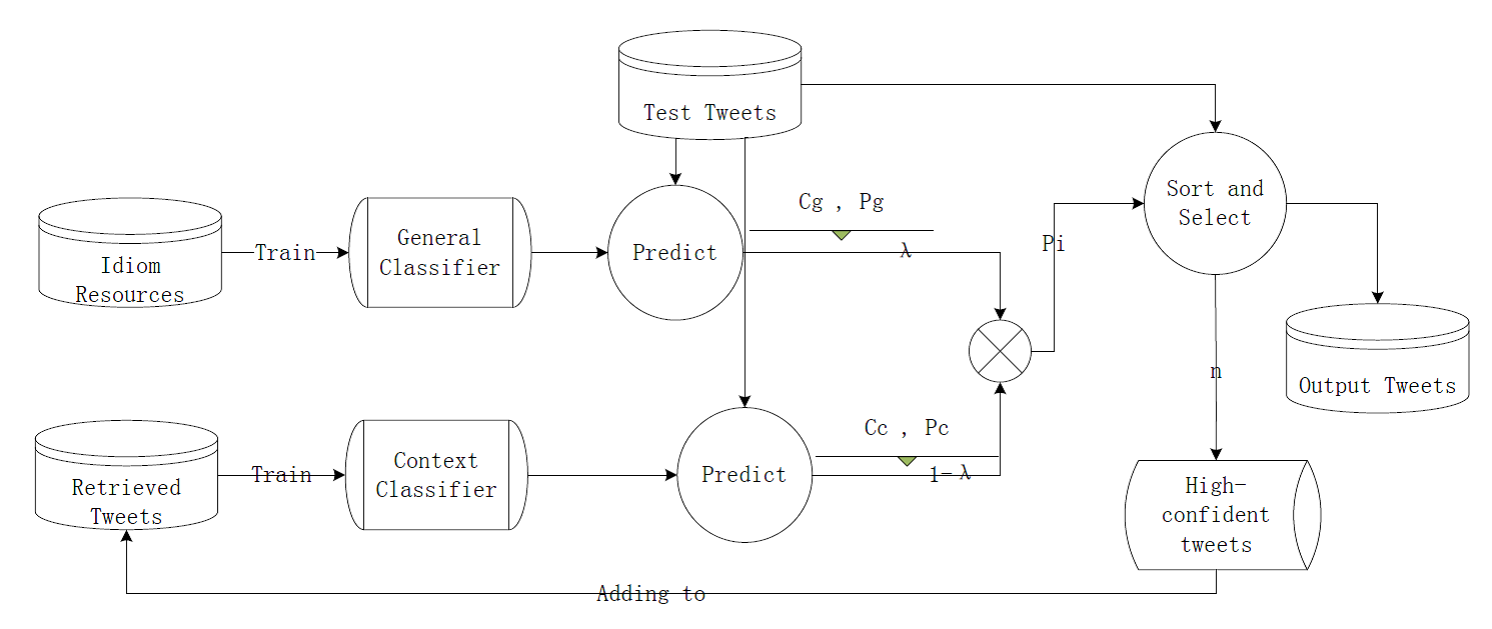
\includegraphics[width=550pt]{4-1.png}
\caption{自举式学习框架}
\label{fig4-1}
\end{figure*}
\end{landscape}
从排序的两组数据中分别取其前$ n $ 条可信度最高的微博数据作为新的微博情感分类器的训练数据加入到训练集中,以逐步提高组合分类器对微博数据的适应性。
整个过程多次循环迭代,直至所有测试数据的情感分类可信度的变化因为小于某个阈值而收敛,最后得到这种自举式学习形成的情感分类器。

总体来说,该框架可以看作是一个协同训练(Co-training)\upcite{marchetti2012learning}的自举式(bootstrapping)机器学习算法,但是该框架并没有需要使用任何标注训练数据,而是从现成的成语词典资源作为训练的起始点,可以看作是一个无监督的学习算法,避免了标注微博数据所需时间和人力开销,对数量庞大的微博数据情感分类问题,该框架更加实用。

\subsection{分类器算法}
\label{classifier}
对于框架中的通用情感分类器和微博情感分类器,本章采用跟Pang等~\upcite{Pang2002}使用的三种机器学习算法:朴素贝页斯(Na\"\i ve Bayes)算法,最大熵(Maximum Entropy)算法以及支持向量机(Support Vector Machine)算法。这三种算法的有效性已经得到Pang等~\upcite{Pang2002}的研究验证,并证明支持向量机取得的性能是最好的(在电影评论数据集上的准确率达到82.9\%),本节对这三种算法进行简单介绍。

\subsubsection{Na\"\i ve Bayes分类器}
\label{bayes}
Na\"\i ve Bayes算法在文本分类任务中是最常用的方法。对于情感分类问题,为了确定一篇文档$ d_{i}$的情感极性性类别$ c_{j} $,Na\"\i ve Bayes算法需要计算后验概率$ P \left(c_{j} \mid d_{i} \right)$。根据Bayes法则和多项式分布,基于每一维特征概率独立性假设,可以得到:
\begin{equation}
\label{e4}
P \left(c_{j} \mid d_{i} \right) = \frac{P \left( c_{j} \right)\prod_{k=1}^{| d_{i} |} P \left( w_{d_{i},k} \mid c_{j} \right)}{\sum_{r=1}^{|C|}P \left( c_{r} \right)\prod_{k=1}^{| d_{i} |} P \left( w_{d_{i},k} \mid c_{r} \right)} \enspace .
\end{equation}
公式中$ r $表示不同的情感类别,$ w $表示文档中出现的词语特征。通过计算不同情感极性类别的后验概率,概率最大极性类别被视为文档 $ d_{i} $的情感极性类别$ c_j $。

\subsubsection{最大熵分类器}
\label{entropy}
最大熵(Maximum Entropy)分类器与Na\"\i ve Bayes分类器一样也是通过计算后验概率来判断文档的情感类别,所不同的是最大熵分类器是计算条件概率:
\begin{equation}
\label{e5}
P \left( c_{j} \mid d_{i}, \overrightarrow{\theta} \right) = \frac{1}{Z}exp \left( \overrightarrow{\theta}, \overrightarrow{f} \left( d_{i},c_{j} \right) \right) \enspace
\end{equation}
其中$ \overrightarrow{\theta} $表示特征向量,$ \overrightarrow{f} \left( d_{i}, c_{j} \right)$表示将训练实例$ \left( d_{i}, c_{j} \right) $映射到特征向量空间的特征函数,$ Z $是归一化因子。
最大熵分类器使用训练数据集$ D $训练学习过程就是解一个最优化问题过程:
\begin{equation}
\label{e6}
\overrightarrow{\theta^{\ast}}=argmax_{\overrightarrow{\theta}}\prod_{i=1}^{|D|} P \left( c_{j} \mid d_{i}, \overrightarrow{\theta} \right) \enspace
\end{equation} 

\subsubsection{SVM分类器}
\label{svm}
支持向量机(SVM)分类器是一种判别式的机器学习方法。支持向量机分类器的训练过程就是发现支持向量所确定的决策平面,该平面能够将训练数据在特征空间上分开为两类,然后使用支持向量确定测试数据的情感极性类别。训练过程是解一个受限的最优化问题:
\begin{equation}
\label{e7}
\begin{aligned}
\overrightarrow{\alpha^{\ast}}=argmin \left( -\sum_{i=1}^{n}\alpha_{i} + \sum_{i=1}^{n} \sum_{j=1}^{n}\alpha_{i}\alpha_{j} x_{i}x_{j}<\overrightarrow{x_{i}},\overrightarrow{x_{j}}> \right)\\
\mbox{Subject to:} \sum_{i=1}^{n}\alpha_{i}y_{i}=0 , 0\leqslant \alpha_{i} \leqslant 1
\end{aligned} \enspace
\end{equation}
其中$ \overrightarrow{x_{i}}$和$\overrightarrow{x_{j}} $为文档特征向量。情感分类问题通常使用线性支持向量机分类器。

\section{实验}
\label{experiment}
为了验证本章提出的无监督自举学习框架的有效性,本节通过在对腾讯微博\footnote{\url{http://t.qq.com/}}展开的情感分类实验进行验证。

\subsection{实验描述}
\label{description}

\subsubsection{数据集}
实验中从成语覆盖比较全的中国教育在线网\footnote{China Education Network:\url{http://chengyu.teachercn.com}}抓取了在线成语词典,经过对词典数据整理和去除中性情感成语条目,最后得到了有8,160个条目的成语数据集,其中褒义(积极情感极性)的成语有3,648条,贬义(消极情感极性)的成语有4,512条,使用这些数据训练来通用情感分类器。
微博情感分类器的训练数据是通过腾讯微博公开API抓取。在2013年4月15日开始到5月15日一个月的时间内,通过监控腾讯微博的实时数据流,查询并抓取了至少含有一条成语的微博,形成120,346条微博数据集。经过筛选和过滤,过滤掉过短微博和噪声微博,最后得到91,268条微博组成的数据集用于训练微博情感分类器。
为了定量评价自举式情感分类器的性能,实验使用了第一届自然语言处理与中文计算会议(Natural Language Processing and Chinese Computing)微博情感分析与语义关系抽取评测(First Chinese tweet Sentiment Analysis and Semantic Relationship Extraction Evaluation)\footnote{中国计算机学会举办:\url{http://tcci.ccf.org.cn/conference/2012/pages/page04_eva.html}}发布的标注微博数据集作为测试数据。评测数据来自腾讯微博,评测数据全集包括 20 个话题,每个话题采集大约1000
条微博(其中积极极性和消极极性各500条),共约20000条微博。
 
\subsubsection{实验配置}
为了能够多角度评价分类器的性能,机器学习中有各种评测指标,由于本实验不是为了比较这些评价指标的不同,因此实验中选择了比较直观的准确率作为分类器性能的评价指标,准确率主要检验分类器对测试数据集分类的准确性。

对于分类器工具,实验选择了自然语言处理的工具箱NLTK(Natural Language ToolKits)\upcite{Loper2002}中的Na\"\i ve Bayes分类器和最大熵分类器,以及常用的Libsvm\upcite{Chang2011}工具包的SVM分类器。
以上分类器中所有的参数设置都经过交叉验证进行了优化。

\subsubsection{评价基准}
为了客观评价自举式分类器的性能,实验设置了三个评价基准用于性能对比。一个是50\%的基本基准,因为实验所用的测试数据集是平衡数据集,所以即便是随机判断的分类器准确率可以达到50\%准确率;第二个基准是一个基于情感词典的情感分类器性能作为对比基准,实验使用的是前面两章构建的SentiHowNet情感词典,通过将每条微博中的包含的情感词的情感极性值累加来计算微博综合情感极性值,然后根据综合情感极性值判断微博的情感极性;第三个基准是使用标注数据进行有监督训练的机器学习方法构建的情感分类器,实验按照Pang等~\upcite{Pang2002}的方法使用测试数据通过5倍交叉验证方式训练了Na\"\i ve Bayes分类器、最大熵分类器以及SVM分类器。

\subsubsection{数据预处理}
中文文本信息不像英文那样具有自然单词结构,因此需要对中文进行分词预处理才能进行词袋特征的抽取。实验使用中科院ICTCLAS分词软件上述所有数据进行分词处理,并进行了停用词过滤\footnote{使用哈工大1208词的停用词表进行过滤}。

\subsection{实验结果}
\label{result}

为了确定公式~\ref{fig4-2}中的最优的$ \lambda $值,首先进行了从0到1对$ \lambda $值遍历实验,实验中分别使用成语数据集和通过远程监督方式获取微博数据集训练分类器,两个分类器对测试数据同时进行情感分类,分类输出的可信度值按照$\lambda $加权组合判断测试数据的极性类别,用准确率评价。每一次遍历$ \lambda $值增加0.1,实验结果如图~\ref{fig4-2}所示。

\begin{figure}[htp]
\centering
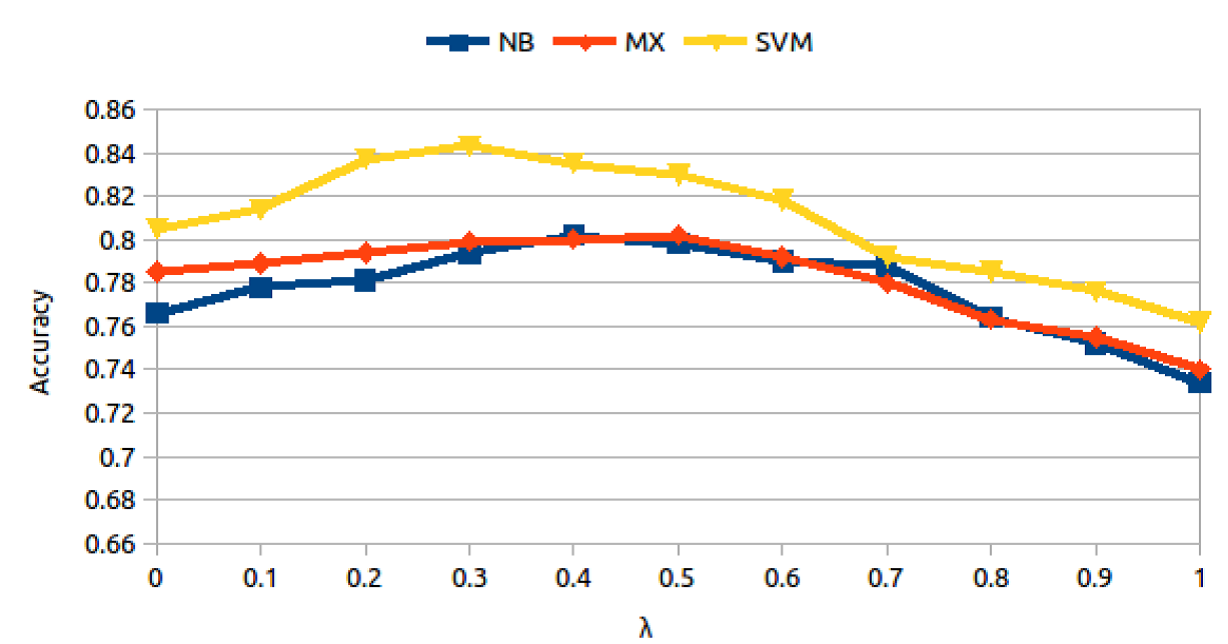
\includegraphics[height=210pt]{4-2.png}
\caption{$ \lambda $值的遍历。}
\label{fig4-2}
%\description{NB代表 Na\"\i ve Bayes分类器,MX代表最大熵分类器,SVM代表支持向量机分类器。}
\end{figure}
从图中可以确定对于三种分类器最优的$ \lambda $值为:对Na\"\i ve Bayes分类器,$ \lambda=0.4 $;对最大熵分类器,$ \lambda=0.5 $;对SVM分类器,$ \lambda=0.3 $。

确定了$ \lambda$后,使用图~\ref{fig4-2}的自举式的学习框架进行训练后对测试数据进行情感分类,分类准确率对比结果如表~\ref{tab4-1}所示。

\begin{table}[htp]
\caption{结果对比表}
\label{tab4-1}
\centering
\begin{tabular}{|l|c|c|c|}
\hline
分类器 &  Na\"\i ve Bayes分类器    &   最大熵分类器    &   SVM分类器    \\
\hline

基于词典方法 & 0.725 & 0.725 & 0.725 \\
\hline
有监督学习方法 & 0.785 & \textbf{0.806} & 0.826 \\
\hline
领域独立部分特征 & 0.734 &  0.740 & 0.762 \\
\hline
领域依赖部分特征 & 0.766 & 0.785 & 0.805 \\
\hline
自举式学习方法 & \textbf{0.802} & 0.802 & \textbf{0.843} \\
\hline
\end{tabular}
\end{table}

根据表中结果,可以得出以下结论:
\begin{itemize}
\item 首先,无论是基于领域独立部分特征的通用情感分类器还是基于领域依赖部分特征的微博情感分类器,准确率都超过了随机基准的50\%准确率,这证明了无论是从那种视角进行分类,两种分类器都是有效的,比随机猜测更准确。因此在没有任何标注数据来训练有监督或半监督分类器的情况下,本章提出特征空间划分假设可以作为微博情感分类的一种有效的方法。
\item 其次,三种通用情感分类器的准确率都比基于情感词典的分类器要高一些,这是因为尽管通用情感分类器和基于词典的分类器潜在假设都是使用情感极性独立于领域的词语来对情感知识进行建模,但是通用情感分类器是经过成语知识资源所抽取的特征训练得到的,而情感词典中情感知识是由单个词语的独立情感极性(值)组成,很多词语的情感极性往往具有一定的歧义;而对于微博情感分类器,准确率比基于词典的分类器和通用情感分类器都要高,因为它是使用微博依赖部分的特征训练得到的,更能适应微博语言环境,测试数据中出现的微博式的“火星语言”越多越能体现出微博情感分类器的性能优越性。
\item 最后,使用自举式学习框架的训练得到的组合分类器显示出了最好的准确率,因为它结合了通用分类器和微博分类器的情感分类性能,其准确率也超过了被Pang等~\upcite{Pang2002}证明的准确率比较高的有监督分类器,这说明本章提出的方法既能很好的利用通用情感表达知识把握微博的总体情感极性,也能照顾到微博语言特有的情感表达方式,准确反映出微博细致的情感极性。
\end{itemize}

\section{小结}
\label{conclusion}
本章首先分析了情感分类问题中面临的领域依赖问题,并针对微博情感分类的领域依赖性问题提出了无监督的自举式学习框架。根据微博情感表达特点,从通用情感表达和微博特有情感表达两个视角对微博情感分类问题进行了重新定义,通过将微博情感分类问题的特征空间进行划分,将整个词语特征空间分为领域独立特征的领域依赖特征两个部分。基于特征空间划分的假设,提出了在两个特征空间分别训练通用情感分类器和微博情感分类器的解决方案,其中通用情感分类器使用现成的成语词典资源作为训练数据进行训练,微博情感分类器使用远程监督方式获取训练数据。为了能够综合两部分特征空间的情感分类作用,设计了自举式的机器学习框架将两种分类器组合起来,形成分类效果更好的情感分类器。实验证明本章所提出的方法性能上超过了基于词典以及有监督机器学习方法,获得了良好的微博情感分类准确性。